\chapter{Theoretical foundations}
\section{Introduction}
Real accelerators operate at a range of beam parameters tailored to specific research purposes. In order to avoid having to set up week-long simulations for each minor change of parameters it is crucial to understand the theory underlying these plasma wakefield phenomena and to investigate to what extent the theoretical predictions match the simulations. Hence, in this chapter, the linear fluid model of plasma wakefield acceleration is introduced and  the equations governing the plasma response to an electron beam driver are derived. We also briefly discuss the non-linear, so-called "blowout", regime which can not be treated perturbatively and is characterised by the expulsion of plasma electrons in a volume behind the bunch. The response to a laser being driven through the plasma, the so-called pondermotive force response, shares many similar features to the theory presented in this chapter but presents other issues such as dissipation and de-phasing in the plasma which will need to be address in the context of the active beam dump. For this reason the theory of laser-plasma interactions will be covered in a subsequent report.  %This model assumes that the electron bunch is ultra-relativistic and that the plasma density is much higher than the bunch density; this will allow us to treat the plasma response as a first-order perturbation to the background density
\section{Linear fluid model }
In this section, we derive the response of a plasma to an electron bunch by considering the plasma electrons as a fluid. We shall make the assumptions:  (i) the initial plasma is uniform and electrically neutral everywhere; (ii) the plasma ions are stationary; (iii) the electron bunch is ultra-relativistic, $v/c\approx 1$, such that the density distribution of the bunch does not evolve significantly as it interacts with the plasma; (iv) the bunch density is much less than the plasma electron density, $n_b<<n_p$.  A beam propagating through a plasma satisfying these conditions is said to be in the \textit{linear regime}. The dynamics of the plasma electrons is governed by the continuity equation
\begin{equation}
\frac{\partial n_p}{\partial t}=-\mathbf{\nabla}\cdot (n_p\vec{v}_p)~,
\end{equation}
where $n_p$ and $\vec{v}_p$ are the plasma electron density density and fluid velocity. This simply ensures charge conservation by imposing that the plasma electron density change in a given volume is due to plasma electrons flowing in or out. The evolution of the electromagnetic fields in the plasma are governed by Maxwell's equations:
\begin{align}
\label{Maxwell1}
&\boldsymbol{\nabla}\cdot \vec{E}=4\pi \rho~,\\
&\boldsymbol{\nabla}\cdot \vec{B}=0~,\\
&\boldsymbol{\nabla}\times \vec{E}=-\frac{1}{c}\frac{\partial \vec{B}}{\partial t} ~,\\
&\boldsymbol{\nabla}\times \vec{B}=\frac{4\pi}{c}\vec{J}+\frac{1}{c}\frac{\partial \vec{B}}{\partial t}~,
\label{Maxwell4}
\end{align}
where, as is convention in plasma physics, we work in CGS units. 
These fields in term determine the response of the plasma fluid through the Lorentz force law:
\begin{equation}
m_e\frac{\partial n_p\vec{v}_p}{\partial t}=en_p\left(\vec{E}+\frac{\vec{v}_p\times \vec{B}}{c}\right)~.
\end{equation}
We now make use of assumption (iv), which allows us to treat the plasma response to a particle beam perturbatively by defining the plasma-electron density $n_p=n_0+n_1$, where $n_0$ is the unperturbed uniform electron density and $n_1\ll n_0$. This perturbation also requires that the change in fluid velocity upon impact with the bunch is small, such that $v_p\ll c$. Substituting this is into the continuity equation  and neglecting terms $\mathcal{O}(n_1/n_0)$ then yields 
\begin{equation}
\frac{\partial^2 n_1}{\partial t^2}= -n_0\frac{\partial (\mathbf{\nabla}\cdot\vec{v}_p)}{\partial t}~.
\label{n''}
\end{equation}
Similarly, substitution into the Lorentz force law simply leaves the electric force:
\begin{equation}
 m_e\frac{\partial \vec{v}_p}{\partial t}= e\vec{E}~,
 \label{lorentz_force_plasma}
\end{equation} %m_en_0\frac{\partial (1+n_1/n_0)\vec{v}}{\partial t}\approx en_0(1+n_1/n_0)\vec{E} \quad \Rightarrow \quad 
which, using Gauss's law, gives
\begin{equation}
\frac{\partial (\mathbf{\nabla}\cdot\vec{v}_p)}{\partial t}= \frac{e^2}{m_e}4\pi (n_1+n_b)
\label{n''2}
\end{equation}
where we have introduced $n_b$ as the density of the electron bunch. Equations (\ref{n''}) and (\ref{n''2}) hence give
\begin{equation}
\frac{\partial^2 n_1}{\partial t^2}+\omega_p^2n_1=-\omega_p^2n_b
\label{ndotdot}
\end{equation}
where 
\begin{equation}
\omega_p=\sqrt{\frac{4\pi e^2n_0}{m_e} }
\label{plasma_frequency}
\end{equation}
is the plasma frequency which determines the magnitude of the plasma-density perturbation. This justifies the stationary-ion assumption (ii) stated above, since for all plasmas the mass of the ions $m_{\text{ion}}>>m_{e}$ the ion-density perturbations will be negligible in comparison to the electron density. Hence the plasma-density perturbation is described by a second-order differential equation with the bunch acting as a source term. We proceed to solve this for a radially symmetric beam by evaluating equation (\ref{ndotdot}) in a reference frame co-moving with the electron bunch \cite{Dawson1959} by defining $\xi=z-ct$ as the position along the bunch as it travels in the $z$-direction. This yields that the co-moving density perturbations  behind with the bunch satisfy
\begin{equation}
-\frac{1}{k_p^2}\left(\frac{\partial^2 }{\partial \xi^2}+k_p^2\right)n_1\left(r,\xi \right)=n_b\left(r,\xi \right) 
\end{equation}  %and causality demands that $n_1\left(r,\xi<0 \right)=0$
where $k_p=\omega_p/c$ is the wavenumber . We evaluate this by finding the Green's function $G\left(\xi,\xi'\right)$, which by definition obeys 
\begin{equation}
-\frac{1}{k_p^2}\left(\frac{\partial^2 }{\partial \xi^2}+k_p^2\right)G\left(\xi,\xi'\right)=\delta\left(\xi-\xi'\right)
\label{density_greens}
\end{equation}
where causality demands that $G\left(\xi<0 ,\xi'\right)=0$ such that
\begin{equation}
G\left(\xi,\xi'\right)=\Theta(\xi-\xi')\left(A(\xi')\sin\left(k_p\xi \right) + B(\xi')\cos\left(k_p\xi \right)\right) 
\end{equation}
where $\Theta(r)$ is the Heavieside step function and the constant $A(\xi')=-k_p\cos(k_p\xi')$ and $B(\xi')=kp\sin(k_p\xi')$ are determined by by requiring continuity at $\xi=\xi'$. The resulting plasma perturbation is therefore
\begin{equation}
\begin{aligned}
n_1\left(r,\xi \right)&=k_p\int_{-\infty}^{\xi}\sin\left(k_p(\xi-\xi')\right)n_b\left(r,\xi' \right) \mathrm{d}\xi'
\end{aligned}
\label{density_perturbation} 
\end{equation} %\int_{-\infty}^{\infty}G\left(\xi,\xi'\right)n_b\left(r,\xi' \right) \mathrm{d}\xi'\\
where we have used the trigonometric identify for $\sin\left(k_p(\xi-\xi'\right))$. Hence the electron bunch induces oscillatory density perturbations in the plasma with a wavelength given by $\lambda_p=2\pi/k_p$. In addition, the magnitude of these perturbation scales linearly with $n_b$, the density of the beam driver, and as $n_0^{1/2}$, the square root of the unperturbed plasma density through equation (\ref{plasma_frequency}). These perturbations set up electromagnetic fields in the plasma behind the beam driver. An understanding of the electromagnetic fields that these perturbations induce is crucial to design a functioning plasma wakefield experiment.
\subsection{Longitudinal Accelerating Field} 
The electric field parallel to the propagation of the beam driver, the so-called longitudinal plasma wakefield, drives particles to either accelerate or decelerate and consequently determines the efficiency of our plasma beam dump. Hence, in this section we derive an expression for this field in the linear regime considered above. 
From Maxwell's equations (\ref{Maxwell1}-\ref{Maxwell4}) it is straightforward to show that the electric field in the plasma obeys a wave equation:
\begin{equation}
\nabla^2\vec{E}-\frac{1}{c^2}\frac{\partial^2 \vec{E}}{\partial t^2}=\frac{4\pi}{c^2}\frac{\partial \vec{J}}{\partial t}+4\pi\boldsymbol{\nabla}\rho~,
\label{E_wave_equation}
\end{equation}
where the change in the current $\vec{J}=\vec{J}_b+\vec{J}_p$ and variations in the charge density $\rho=\rho_b+\rho_p$ act as source terms. Furthermore, we have from equation (\ref{lorentz_force_plasma}) that 
\begin{equation}
\frac{\partial \vec{J}_p}{\partial t}=\frac{e^2 n}{m_e}\vec{E}~.
\end{equation}
Substituting this into equation (\ref{E_wave_equation}), together with the an ultra-relativistic beam current $\vec{J}_b=c\rho_b\hat{\vec{z}}$, gives that the longitudinal wakefield $E_z$ satisfies
%\begin{equation}
%\left(\nabla^2-\frac{1}{c^2}\frac{\partial^2}{\partial t^2}-k_p^2\right)\vec{E}=\frac{4\pi}{c}\frac{\partial \rho_b}{\partial t}\hat{\vec{z}}+4\pi\boldsymbol{\nabla}\left(\rho_b+\rho_p\right)
%\end{equation}
\begin{equation}
\left(\nabla^2-\frac{1}{c^2}\frac{\partial^2}{\partial t^2}-k_p^2\right)E_z=\frac{4\pi}{c}\frac{\partial \rho_b}{\partial t}+4\pi\frac{\partial}{\partial z}\left(\rho_b+\rho_p\right)~,
\label{Ez_wave_equation}
\end{equation}
where $k_p=\omega_p/c$ is the plasma wave number. To solve this we assume that $E_z$ is radially symmetric and write the Laplace operator in cylindrical polar coordinates, $\nabla^2=\nabla^2_{\perp}+\partial^2_z$, where the transverse component
\begin{equation}
\nabla_{\perp}^2=\frac{1}{r}\frac{\partial }{\partial r}r\frac{\partial }{\partial r} +\frac{1}{r^2}\frac{\partial^2 }{\partial \phi^2} ~.
\end{equation}
Furthermore, the derivation is simplified by working in Fourier transform space, where
\begin{equation}
E_z(\xi)=\frac{1}{2\pi}\int_ {-\infty}^{\infty}\wtilde{E}_z(k)e^{ik\xi}\mathrm{d}k~,
\end{equation}
and similarly for $\rho_b$ and $\rho_p$. Equation (\ref{Ez_wave_equation}) then simplifies to
%\begin{equation}
%\left(\frac{\partial^2 }{\partial z^2}-\frac{1}{c^2}\frac{\partial^2 }{\partial t^2}\right)E_z(\xi)=0
%\end{equation}
%and
%\begin{equation}
%\frac{4\pi}{c}\frac{\partial {\rho}_b}{\partial t}+4\pi\frac{\partial }{\partial z}\left({\rho}_b+{\rho}_p\right)=-4\pi i k\wtilde{\rho}_b+4i k\pi\wtilde{\rho}_b+4i k\pi\wtilde{\rho}_p=4i k\pi\wtilde{\rho}_p
%\end{equation}
%which gives 
\begin{equation}
\left(\nabla^2_{\perp}-k^2_p\right)\wtilde{E}_z\left(\xi\right)=4\pi i k\wtilde{\rho}_p~,
\end{equation}
We note that in this form the two contributions from the beam, $\vec{J}_b$ and $\rho_b$, have cancelled each other out. This is because the beam velocity was set to $\beta=1$, such that the electric field of the beam itself is purely in the radial direction \citep{Gessner2016}. The effect of the beam is however represented in the plasma modulations $\wtilde{\rho}_p$ through equation (\ref{density_perturbation}). Given that experimentally the beam density is often known, and the plasma perturbations can only be inferred from data, it is convenient to write this relationship in a compact form by taking the Fourier transform of equation (\ref{ndotdot}), such that
%\begin{equation}
%\frac{\partial^2{\rho}_p}{\partial t^2}+\omega_p^2{\rho}_p=-\omega_p^2{\rho}_b \quad \Rightarrow\quad
%-k^2\wtilde{\rho}_p+k_p^2\wtilde{\rho}_p=-k_p^2\wtilde{\rho}_b 
%\end{equation}
%which gives 
%\begin{equation}
%\wtilde{\rho}_p=\frac{k_p^2}{k^2-k_p^2}\wtilde{\rho}_b~.
%\end{equation}
%At this point it should be noted that a setting the beam velocity to $\beta=1$ before solving this equation, as we have done here, is technically not valid...... However, the effect of this is altogether negligible in our case (calc extra term from their paper).\\
\begin{equation}
 \left(\frac{\partial^2 }{\partial r^2}+\frac{1}{r}\frac{\partial }{\partial r} -k^2_p\right)\wtilde{E}_z
=4\pi ik_p^2 \frac{k}{k^2-k_p^2}\wtilde{\rho}_b
\label{diffeq_in_transformspace}
\end{equation}
which we define in a compact form as $\mathscr{L}\wtilde{E}_z= \wtilde{f}(r,k)$. This is the Fourier transformed version of equation (\ref{Ez_wave_equation}), which has the advantage of the source term $\wtilde{f}(r,k)$ being a function of the beam density alone. Hence by solving this this PDE we can find $E_z$ through an inverse Fourier transform. This is again done by finding its Green's function, $G(\vec{r},\vec{r}')$, which in cylindrical coordinate satisfies
\begin{equation}
\mathscr{L}G(\vec{r},\vec{r}')=\frac{1}{r}\delta(r-r')\delta(\phi-\phi')\delta(z-z')
\end{equation}
where the delta function has been written in cylindrical polar coordinates. Since the PDE is radial we can write the Green's function as
\begin{equation}
G(\vec{r},\vec{r}')=G_r(r,r')\delta(\phi-\phi')\delta(z-z')
\end{equation}
which leads to 
\begin{equation}
\mathscr{L}G_r(r,r')=\frac{1}{r}\delta(r-r')
\label{greens_diff_eq}
\end{equation}
where left-hand side is the modified Bessel function of order zero \cite{Jackson1962}. Consequently, the Green's function is formed by linear combinations of the modified Bessel functions of order zero, denoted by $K_0$ and $I_0$: %\todo{Standard Bessel function with complex arguments} the linearly independent, 
\begin{equation}
G\left(r,r'\right)=\left\{ \begin{array}{ll}
A(r')(A_1 I_0(k_pr)+B_1K_0(k_pr)) &,~ 0<r<r'\\
B(r')(A_2 I_0(k_pr)+B_2K_0(k_pr))  &,~ r'<r<\infty~.
\end{array}\right.
\end{equation} %since $K_0(k_pr)\to \infty$ as $r\to 0$ and $I_0(k_pr)\to \infty$ as $r\to \infty$.
By requiring that the two parts of this expression each satisfy one of the boundary conditions, namely that the functions are finite at $r=0$ and tend to zero as $r\to\infty$, we have that $B_1=A_2=0$. Continuity in $G(r,r')$ at $r=r'$ further gives that 
\begin{equation}
G\left(r,r'\right)=A_0\left\{ \begin{array}{ll}
I_0(k_pr)K_0(k_pr') &,~ 0<r<r'\\
I_0(k_pr')K_0(k_pr)  &,~ r'<r<\infty
\end{array}\right.
\end{equation}
where $A_0$ is a constant of proportionality that we find by integrating %$\mathscr{L}G(r,r')=\delta(r-r')/r$ 
equation (\ref{greens_diff_eq}) across the interval $r\in\left[r'-\epsilon, r'+\epsilon \right]$. This expression needs to be satisfied for all $\epsilon$, including the limit as $\epsilon\to 0$, such that
%\begin{equation}
 %\lim_{\epsilon\to 0}\int_{r'-\epsilon}^{r'+\epsilon}\left(\frac{\partial^2 G}{\partial r^2}+\frac{1}{r}\frac{\partial G}{\partial r} -k^2_pG\right)\mathrm{d}r= \lim_{\epsilon\to 0}\int_{r'-\epsilon}^{r'+\epsilon}\frac{1}{r}\delta(r-r')\mathrm{d}r
 %\end{equation}
\begin{equation}
\lim_{\epsilon\to 0}\int_{r'-\epsilon}^{r'+\epsilon}\mathscr{L}G_r(r,r')\mathrm{d}r= \lim_{\epsilon\to 0}\int_{r'-\epsilon}^{r'+\epsilon}\frac{1}{r}\delta(r-r')\mathrm{d}r
 \end{equation}
 %\lim_{\epsilon\to 0}\Big[\frac{1}{k_p}\frac{\partial G}{\partial r} \Big]_{z-\epsilon}^{z+\epsilon}=
% \begin{equation}
 %\frac{A_0}{k_p} \left.\left(I_0(k_pr')\frac{\partial K_0(k_pr)}{\partial r}-\frac{\partial I_0(k_pr)}{\partial r}K_0(k_pr')\right)\right|_{r=r'} =\frac{1}{r'}~.
 %\end{equation}
%This equality must hold for all finite values of $r'$. Hence, following an approach by Jackson \citep{Jackson1962}, we evaluate this expression for $k_pr'\gg 1$, where $I_0$ and $K_0$ take the limiting forms: 
%\begin{equation}
%I_0(k_pr')\to \frac{1}{\sqrt{2\pi k_pr'}}e^{k_pr'} \quad \text{and} \quad K_0(k_pr')\to \sqrt{\frac{\pi}{2k_pr'}}e^{-k_pr'}
%\end{equation}
which implies that $A_0=-1$ and that
\begin{equation}
G\left(r,r'\right)=- I_0(k_pr)K_0(k_pr')\Theta(r'-r)-I_0(k_pr')K_0(k_pr)\Theta(r-r')~.
\end{equation}
We can thus find $\wtilde{E}_z$ from 
\begin{equation}
\wtilde{E}_z(r,k)=\int_{0}^{\infty}G\left(r,r'\right)f(r',k)r'\mathrm{d}r'
\end{equation}
and then perform an inverse Fourier transform to find the co-moving longitudinal wakefield:
%\begin{equation}
%E_z(r,\xi)=\frac{1}{2\pi}\int_ {-\infty}^{\infty}\wtilde{E}_z\left(r,k\right)e^{ik\xi}\mathrm{d}\xi
%\end{equation}
%Doing this yields 
\begin{align}
E_z(r,\xi)&=-{2ik_p^2}\int_{-\infty}^{\infty}\frac{ke^{ik\xi}}{k^2-k_p^2}\mathrm{d}k\int_0^{\infty}G\left(r,r'\right)\wtilde{\rho}_b(r')r'\mathrm{d}r'
\label{e_z}
\end{align}
%For a known beam distribution $\rho_b(r,\xi)$ (add $\xi$ in all previous expressions?) this expression can be used to compute the resulting longitudinal electric field. We shall now proceed by calculating this for a bi-Gaussian bunch distribution. To do this, we could compute the electric field from the Green's function directly and then carrying out the inverse Fourier transform, or we could choose to first compute the field due to a point-particle and then convolving it with the bi-Gaussian distribution. We proceed by doing the latter by following the approach of Dawson \cite{Katsouleas1987} ; we choose a charge distribution with radial symmetry and a delta function in the $z$-direction to match our Green's function.
For a known beam distribution $\rho_b(r,\xi)$ this expression can be used to compute the resulting longitudinal electric field. Of particular interest to us is the field induced by the propagation of an electron bunch that is Gaussian in both the transverse and longitudinal direction, a so-called bi-Gaussian bunch. To compute this we follow an approach by Dawson \cite{Katsouleas1987} and first evaluate the field due to a point-particle and then convolve it with our bi-Gaussian driver. We choose a radially symmetric point-particle distribution ${\rho}_{0}(r,\xi)$ to match our Green's function:
\begin{align}
{\rho}_{0}(r,\xi)=-\frac{e}{2\pi r}\delta(r-r')\delta(\xi) %\quad \Rightarrow\quad  \wtilde{\rho}_{b_0}(r,k)=\int_ {-\infty}^{\infty}\rho_b(r,\xi)e^{-ik\xi}\mathrm{d}\xi=\frac{e}{2\pi r}\delta(r-r')
\end{align}
Substituting the Fourier transform of this into equation (\ref{e_z}) and performing a contour integrating in k-space yields 
\begin{equation}
E_z(r,\xi)=2ek_p^2\cos(k_p\xi)G\left(r,r'\right)\Theta(\xi)~,
\label{singe-particle-wake}
\end{equation}
where $\Theta(\xi)$ ensures causality is preserved. This is the so called single-particle wake function \cite{Katsouleas1987}. The longitudinal electric field resulting from an arbitrary radially-symmetric source distribution $n_b(r,\xi)$ is now given by convolving the source by the single-particle wake function:
\begin{align}
E_z(r,\xi)=2ek_p^2\int_0^{2\pi}\mathrm{d}\phi  \int_{-\infty}^{\infty} \cos(k_p(\xi-\xi'))\Theta(\xi-\xi')\mathrm{d}\xi' \int_{0}^{\infty}G\left(r,r'\right) n_b(r',\xi')r'\mathrm{d}r'
\end{align}
%\begin{equation}
%\wtilde{E}_z(r,k)=-2eik_p^2\frac{k}{k^2-k_p2}G\left(r,r'\right)
%\end{equation}
%which satisfies (\ref{diffeq_in_transformspace}), as can be shown by integrating across the discontinuity and taking the limit to zero, and then gives
%\textcolor{red}{But my Green's function has a $A=-1$ as constant and not $A=4\pi$ as Bonatto and Gessner}\\The electric force is thus $F_z(r,\xi)=-eE_z(r,\xi)$. 
To compare with simulations and experiments we now choose to convert from CGS to SI units by having $e^{\text{CGS}}\to e^{SI}/\sqrt{4\pi\epsilon_0}$. The longitudinal wakefield in SI units (J/m) is thus
\begin{equation}
E_z(r,\xi)=\frac{e k_p^2}{\epsilon_0} \int_{-\infty}^{\xi} \cos(k_p(\xi-\xi'))\mathrm{d}\xi' \int_{0}^{\infty}G\left(r,r'\right) n_b(r',\xi')r'\mathrm{d}r'
\label{longitudinalforce}
\end{equation}
To test the validity of the linear fluid model as well as highlight some key features of the longitudinal wakefield we will calculate this field numerically for a 1 GeV bi-Gaussian bunch with a density of the form
\begin{equation}
n_b(r,\xi)=\frac{N_b}{(2\pi)^{3/2}\sigma_r^2\sigma_{\xi}}e^{-\xi/(2\sigma_{\xi}^2)-r/(2\sigma_{r}^2)}
\label{bigaussian}
\end{equation}
\begin{figure}[!ht]
\centering
\includegraphics[width=0.8\textwidth]{longitudinal2d_final}
\label{transverse_plot}
\caption{Two-dimensional simulation plot of the co-moving longitudinal electric field in the linear regime, $n_p=100n_b$. The electron bunch (not shown) is centred on $\xi=0$ and moves to the right.}
\end{figure}
\clearpage
where $N_b$ is the number of electrons in the bunch and $\sigma_{\xi}$ and $\sigma_r$ are the standard deviation of the bunch in the longitudinal and transverse direction. At this stage we will also compare these calculations to equivalent two-dimensional PIC simulations using EPOCH, as described in chapter 2.  We choose a plasma density $n_p=100n_b$ to ensure that the electron beam is in the linear regime. We also set the bunch dimensions to $\sigma_{\xi}=\sigma_r=5~\mu\text{m}$ and $N_b=10^6$ to allow for later comparisons with the simulations presented in chapter 4. The beam dump that we have in mind will not necessarily have the beam in the linear regime, however the linear-regime simulations in this chapter will function as a benchmark for the validity of the linear model. The resulting two-dimensional co-moving longitudinal wakefield from this simulations is shown in figure (\ref{transverse_plot}), where the beam has propagated only $200~\mu\text{m}$ to the right to minimize bunch distortions. Remembering that these fields are induced by electron density modulations this plot clearly shows the oscillatory density-perturbations described by equation (\ref{density_perturbation}). To allow for comparison with equation (\ref{longitudinalforce}) we extract the data for the electric field at $Y=0$ and compare to calculations at $r=|y|=0$, the result of which is shown in figure \ref{theory_vs_simulation}. We note that the theoretical calculations and the simulations are indeed in good agreement, with the linear model predicting both the amplitude and the wavelength of the induced plasma wakefield. We also note that the electric field is positive along the bunch, implying that there is a decelerating force on the electron bunch. We can also identify some of the features that previous studies have found. In particular, the energy chirp found by Wu et. al, figure \re{Wu}, can be explained by the fact that both theory and simulation predict that the head of the bunch, $\xi>0$, should experience a near-zero electric field. As a result, energy loss should only occur through scattering mechanisms, which are entirely negligible compared to the effect of this wakefield \cite{Wu2010}. We may furthermore predict that this method can not fully deplete the energy of the beam on its own. For, assuming that the electric field maintains its form as the beam propagates, as soon as particles lose enough energy to fall behind the rest of the bunch, they will end up in a region of negative electric field, $-25<\xi<-15 ~\mu\text{m}$, and subsequently get re-accelerated. One method for dealing with this was described in chapter 1, whereby Wu et al. \cite{Wu2010}. simulated the use of foils to prevent particles reaching the re-acceleration region. The other method, proposed by Hanahoe et al. \cite{Hanahoe2017} was to let the beam propagate through an increasing plasma density. Although this method has not been simulated so far, if the proposed experiments at FLASHForward at DESY in 2019 include the possibility to test this proposal this method will need to be explored further in the upcoming report. This method utilizes the transverse wakefields, which we cover below for completeness. 



%This might at first sight appear unsurprising, since if the bunch moved through a solid material it would loose energy as well, and as the bunch moves through the plasma it displaces electrons which transfers kinetic energy to the plasma. The surprise here however is the uneven way in which the plasma electrons rearrange themselves. Each electron displaces plasma electrons, and each electron transfers a small amount of energy to the plasma electrons, the plasma electrons arrange themselves in such a way as to collective create a large electric field in the middle of the bunch. So even though each electron transfers some energy kinetically, the ones in the middle will lose a lot more energy through this decelerating  electric field which all the electrons in the bunch has contributed to setting up. 







%For this reason this is referred to as collective deceleration. 

\begin{figure}
\centering
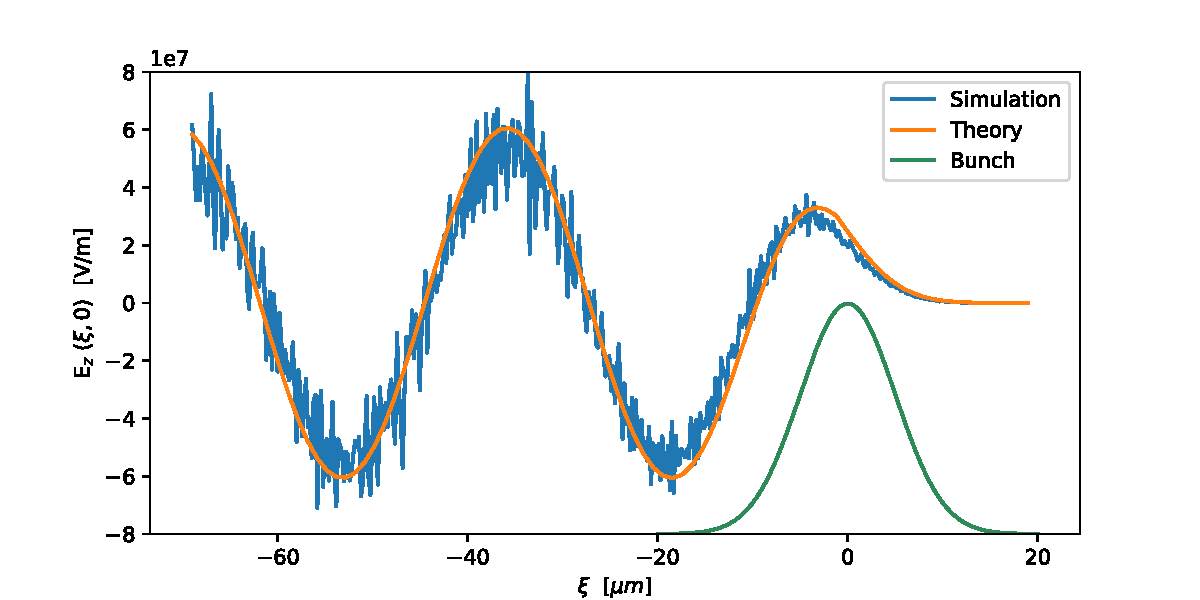
\includegraphics[width=0.8\textwidth]{longitudinal_theory_vs_simulation.pdf}
\caption{Simulation vs. theory for linear regime with $n_p/n_b=100$. }
\label{theory_vs_simulation}
\end{figure}
\clearpage
\subsection{Transverse Field} 
An ultrarelativisitic electron bunch will be highly contracted in the direction of propagation relative to the plasma electrons in the 'lab' frame. Assuming $\beta=1$ as before the electric field due to the bunch is purely radial, $E_r$. In addition, the magnetic field due to the charge is azimuthal, $B_{\theta}$. The resulting transverse wakefield $W_{\perp}=E_+-cB_{\theta}$ experienced by a realtivisit particle due to the wake is given by the \textit{Panofsky-Wenzel theorem}\cite{Vaganian1995}, which says that the transverse wakefield at a position $\xi=z-ct$ behind the head of the bunch is related to the longtiduinal wakefield $W_{\parallel}$ via
\begin{equation}
\frac{\partial W_{\perp} }{\partial z}=\frac{\partial W_{\parallel} }{\partial r}~.
\end{equation} 
Since $W_{\parallel} =E_z$ this gives a transverse wakefield
\begin{equation}
W_{\perp}(\xi)=\int \frac{\partial E_z }{\partial r}\mathrm{d}z~.
\end{equation}
The transverse force on a bi-Gaussian bunch can now by found by applying this expression to on the longitudinal single-particle wakefield (\ref{singe-particle-wake}) and then performing the same convolution as above \cite{Katsouleas1987, Mira2017}, which yields 
\begin{equation}
F_r(r,\xi)=-\frac{e^2 k_p}{\epsilon_0} \int_{-\infty}^{\xi} \sin(k_p(\xi-\xi'))\mathrm{d}\xi' \int_{0}^{\infty}\frac{\partial G\left(r,r'\right)}{\partial r} \frac{n_b(r',\xi')}{\partial r'}
r'\mathrm{d}r'
\end{equation}
%where 
%\begin{equation}
%n_b(r,\xi)=\frac{N_b}{(2\pi)^{3/2}\sigma_r^2\sigma_{\xi}}e^{-\xi/(2\sigma_{\xi}^2)-r/%(2\sigma_{r}^2)}
%\label{bigaussian}
%\end{equation}
%and 
%\begin{equation}
%G\left(r,r'\right)=- I_0(k_pr)K_0(k_pr')\Theta(r'-r)-I_0(k_pr')K_0(k_pr)\Theta(r-r')~.
%\end{equation}
\begin{figure}
\centering
\includegraphics[width=0.8\textwidth]{transverse_2d_plot}
\label{transverse_plot}
\caption{•}
\end{figure}

From this we note that the radial field exhibits the same oscillatory behaviour that we have seen before and that the phase of the transverse and longitudinal fields differ by $\pi/2$. This is of particular importance to plasma wakefield accelration experiments, since it implies that there will be a region which is simultaneously accelrating and focusing, enabling high acceleration of narrow beams. Hanahoe et al. was able to use a similar appraoch to show that by employing a varying density one could find that reaccelration of particles that had fallen behind the bunch occurred in a defocusing region. Thereby forcing the particles outwards, where they were subsequently decelerated through ordinary scattering. Figure \ref{transverse_plot}.\\
%Firstly, the radial field at $r=0$ is zero since 
%begin{equation}
%\left.\frac{\partial G\left(r,r'\right)}{\partial r} \right|_{r=0}=\frac{k_p}{2} I_1(0)K_0(k_pr')=0
%\end{equation}
%\begin{figure}
%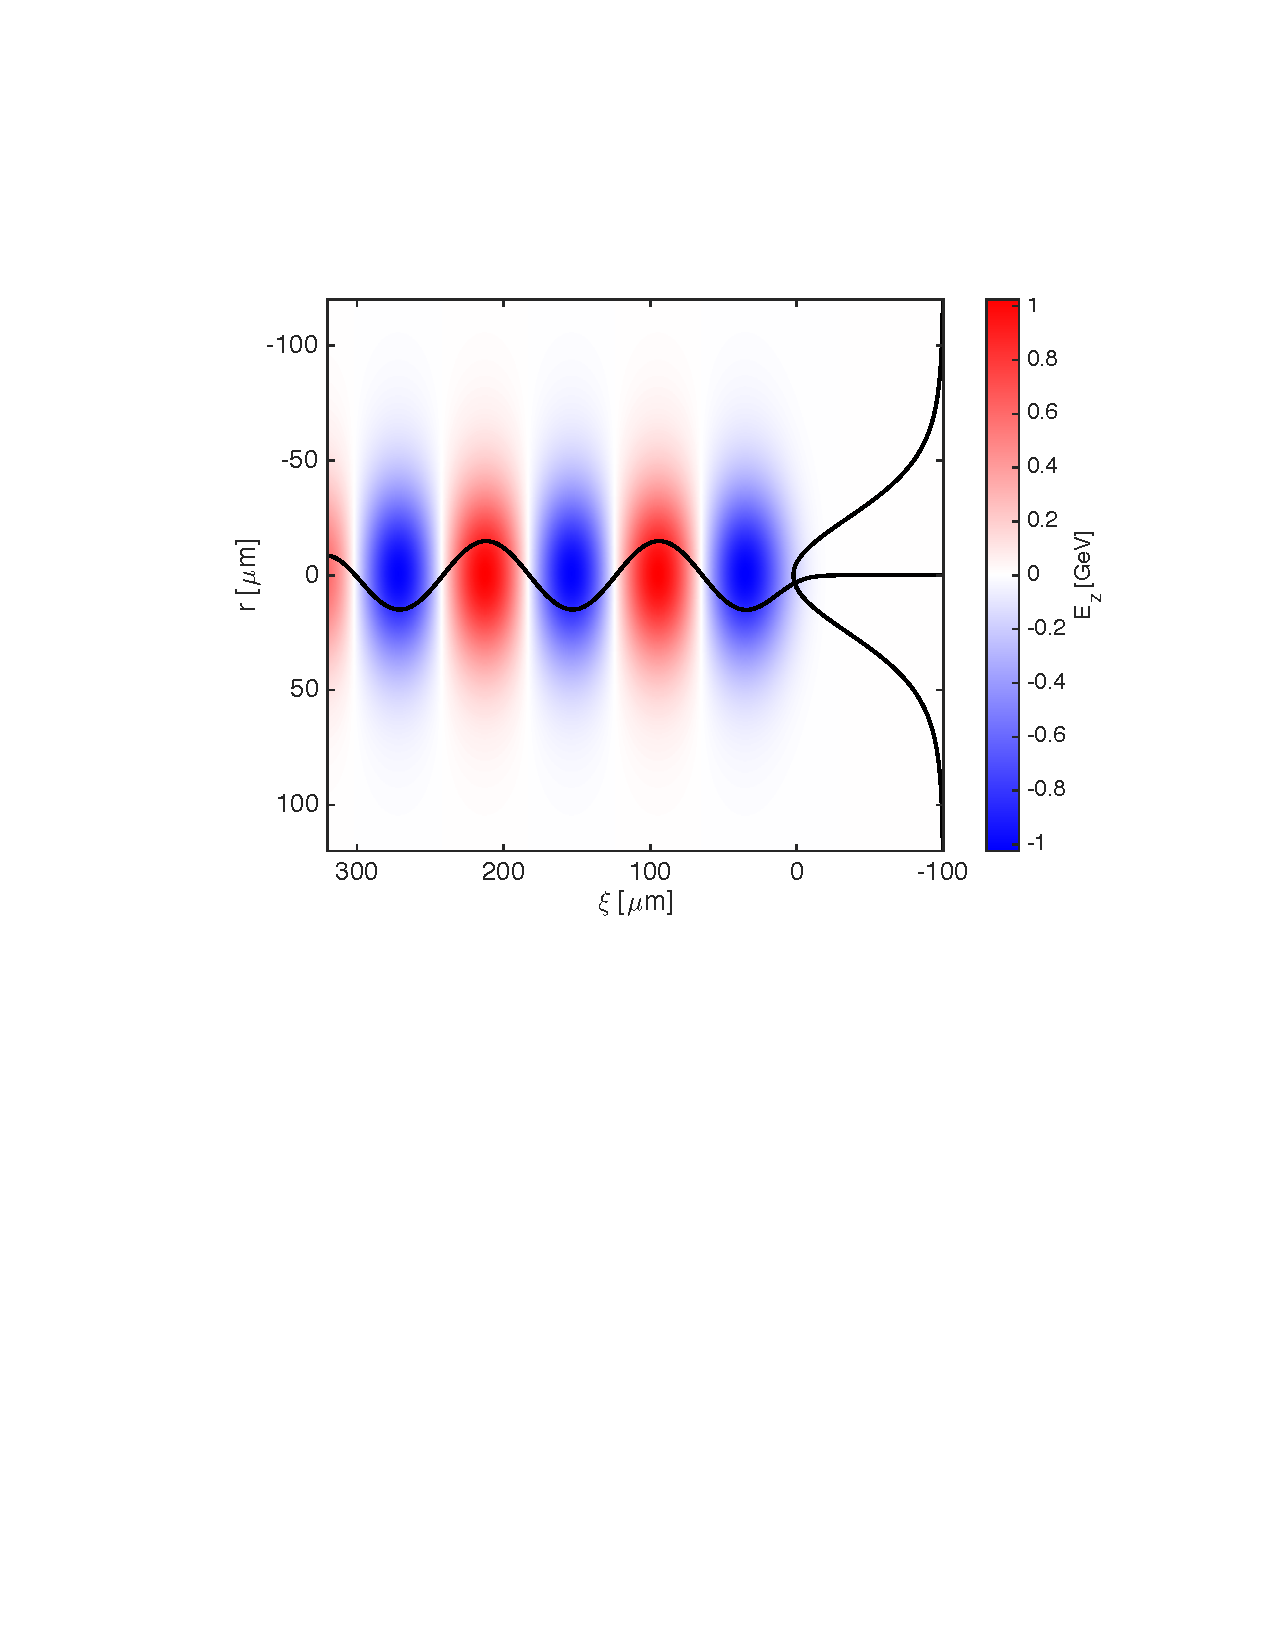
\includegraphics[width=0.49\textwidth]{longitudinal_gessner}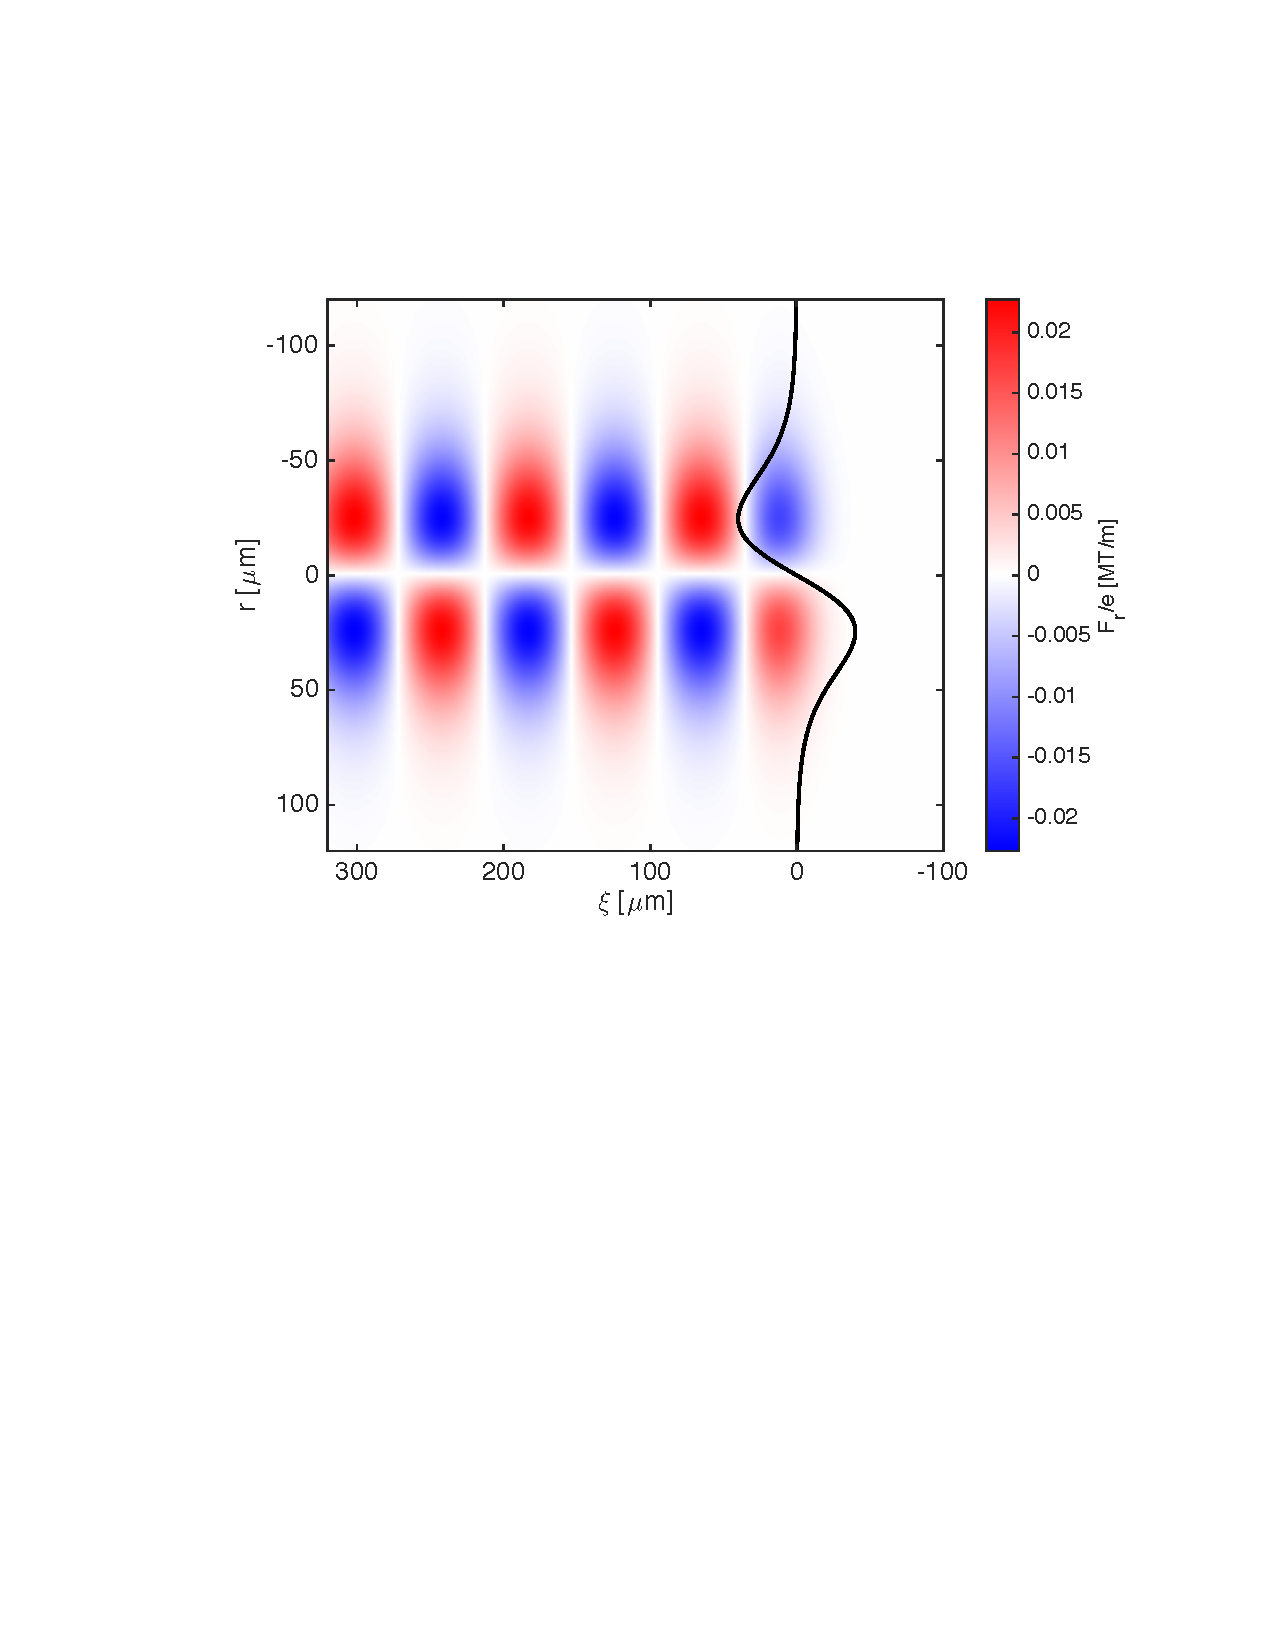
\includegraphics[width=0.49\textwidth]{transverse_gessner}
%\end{figure}
\begin{figure}
\centering
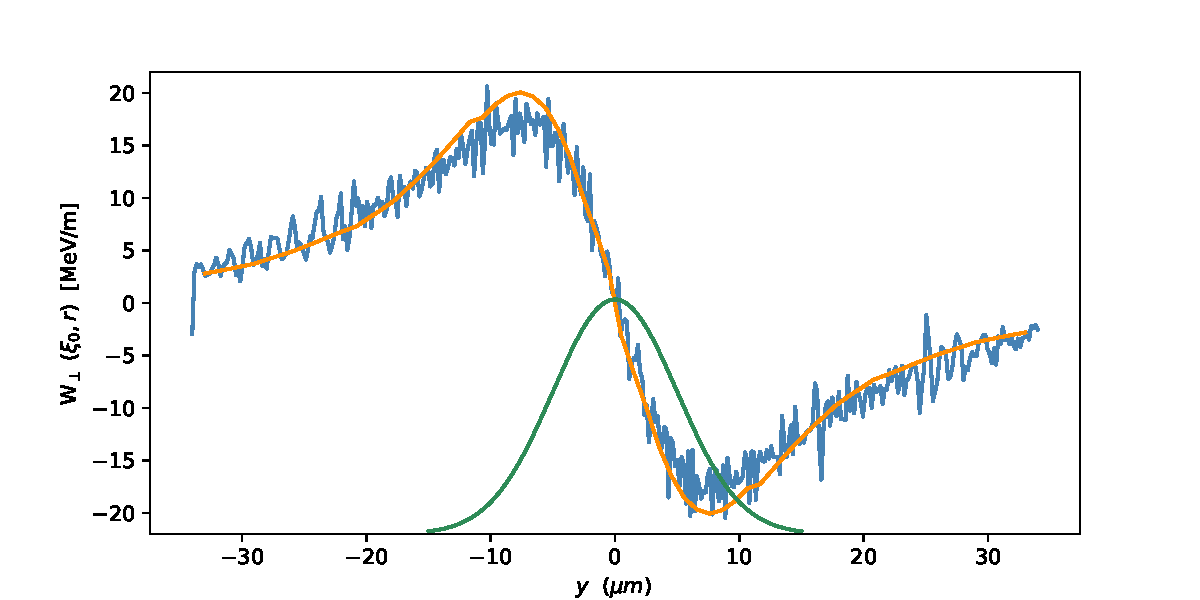
\includegraphics[width=\textwidth]{test.pdf}
\caption{Transverse force - theory vs. simulation}
\end{figure}

\subsection{Collective Plasma Deceleration -- Linear regime }
As described above parts of the electron bunch can be in either accelerating or decelerating regions. The parts of the bunch that are in a decelerating region will lose energy; this is the general idea behind a plasma beam dump. Since we can calculate the electric field at any position ($\xi,r$) along the bunch we can estimate the energy loss by calculating the work carried out by the longitudinal electric field. Since the beam is assumed to be rigid in the linear regime this does not take into account accelerated particles. This is the approach taken by Bonatto et al. to estimate the distance required to dump various beams in passive or active plasma beam dumps \citep{Bonatto2016}, and as we shall see in section XXX this approach provides good agreement with simulations.\\
The rate of energy change with propagation distance of a particle at position $(r,\xi)$ in the bunch after travelling is given by the force exerted on the particle by the longitudinal electric field:
\begin{equation}
\frac{\mathrm{d}U_p}{\mathrm{d}s}=-eE_z(r,\xi)
\end{equation}
where we have assumed that there occurs no modulation of the particle bunch as it traverses the plasma, hence the electric field is only a function of the position in the bunch $E_z(r,\xi)$ and not the propagation distance $s$. Integrating over the propagation distance then gives the energy of one particle in the beam at position $(r,\xi)$ after travelling a distance s:
\begin{equation}
U_e(r,\xi,s)=U_e(r,\xi,0)-seE_z(r,\xi)
\end{equation}
from which multiplication by the beam number density $n_b(r,\xi)$ and integration over the volume of the bunch gives the total energy of all particles in the bunch after propagation distance s
\begin{equation}
U(s)=\int  U_e(r,\xi,0)n_b(r,\xi)r\mathrm{d}r\mathrm{d}\xi\mathrm{d}\phi-se\int E_z(r,\xi)n_b(r,\xi)r\mathrm{d}r\mathrm{d}\xi\mathrm{d}\phi
\label{energy_loss_bonatto}
\end{equation}
where $E_z$ and $n_b$ are found from equations (\ref{longitudinalforce}) and (\ref{bigaussian}). A program to compute this numerically has not yet been implement, but we endeavour to do so in the latter part of this project to allow for comparisons between the linear theory and simulations.
%\subsection{Notes Bonatto}
%Rate of change due to the longitudinal electric field acting on an electron beam, i.e position beam in the decelerating region of the wakefield.\\
%"the beam only experiences its self-excited wakefield."\\
%In the passive beam dump, are we essentially slowing down a "drive bunch" without having a witness bunch behind to get accelerated?\\
%It is probaly better to u se gamma as in Bonatto's paper, to make it easier to explain total beam energy integral. Basically integrate over all particles.\\
%$U=\gamma m_ec^2$
%\begin{equation}
%-\frac{\mathrm{d}U}{\mathrm{d}s}=(F_e)_z=eE_z
%\end{equation}
%where $s$ is the distance travelled in the plasma and $U$ is the energy of a particle in the beam at position $\xi$. 
%for ultra relativistic beams, $\beta\sim 1$, the longitudinal electric field is a function of the position along the bunch $\xi=z-ct$ and not $z$ explicitly. 
%\begin{equation}
%U(s,\xi)=U_0-esE_z(\xi)
%\end{equation}
%The total energy of the beam after travelling a distance $s$ is then found by integrating across all the particles in the beam, which is integrating across $\xi$ since analysis is in 1-D.
%\begin{equation}
%\mathcal{U}(s)=U_0\int_{-\infty}
%\end{equation}

%We will proceed by calculating the gamma factor of a given particle in the beam who's energy we wish to compute.
%\begin{equation}
%\gamma(s,\xi)=\gamma_0-esE_z(\xi)
%\end{equation}

%Based on the work of Lu et. al \citep{Lu2006}, wherein it was shown that the predictions from the linear models perform well even in the non-linear regime, it is of interest to compute the energy loss in the linear regime. 

%\section{Non-linear Regime} 
%Lower density, larger plasma response, not possible to describe perturbatively. Hamiltonian approach taken by Lu. et al []\\
%Self-injection?